\chapter{Cahier des charges}
	
	\section*{Introduction}

		Ce cahier des charges contient les objectifs ainsi que les différentes
	méthodes employées dans le cadre du projet MI S3.
	
	\section{Objectif}
	
		L'objectif du projet est la génération de paroles à partir d'un texte
	(Text to Speech, TTS). Les données seront extraites à partir d'audio-books
	libres de droit.
	
		Ce projet peut se diviser en deux catégories: la création de la base de
	données et la création de la parole à partir de cette dernière.
	
		De nombreux ajouts sont possibles.
		
	\section{Génération de la base de donnée}
	
	Dans cette section, nous discutons de comment nous allons générer notre
	base de donnée.
	
		\subsection{Récupération des données}
		
		Les données sont des audio-books libres de droit venant du projet Librivox
	\footnote{\url{https://librivox.org/}}.
	Ces audio-books sont au nombre de 9350. Si on compte environ 100 Mo 
	l'audio-book, cela représente une quantité audio d'environ 935 Go.
	Nous ne travaillerons au départ que sur une petite portion de ces données.
	Nous ne travaillerons que sur les audio-books en anglais et prononcés par une
	seule personne.
	
	~
	
	Le texte provient du projet 
	Gutenberg\footnote{\url{http://www.gutenberg.org}}.
	Pour l'instant la récupération de l'audio book et du texte correspondant
	sera fait à la main. Une récupération via un crawler est envisageable.
	
		\subsection{Segmentation de l'audio}
		
	Une fois l'audio récupéré il s'agit de découper la bande sonore en mots
	et de faire la correspondance avec le texte.

	~	
	
	Il semble plus facile de traiter phrase par phrase, puisque cela va 
	permettre d'éviter l'accumulation d'erreur. Il faut donc commencer par
	séparer l'audio en plusieurs phrases. Là encore une séparation manuelle est
	envisageable, mais il serait intéressant d'automatiser complètement cette
	étape. De plus comme la quantité de donnée est très importante, on peut
	très bien jeter toutes les données dont nous ne sommes pas sûrs. Par exemple
	ne traiter que la première phrase de chaque chapitre (en effet, l'audio est
	séparé en chapitre).
	
	~	
	
	Pour la segmentation en mots on peut envisager d'étudier les micro-coupures
	entre chaque mots. Pour un mot on obtient plusieurs sons, on peut envisager de
	prendre uniquement les sons similaires pour éliminer les erreurs.
	
	~
	
	On peut également avoir une approche non supervisée~\cite{ludusan:hal-01026368}:
	\begin{itemize}
		\item regrouper les sons similaires par paire
		\item regrouper les paires en \textit{cluster} par F-score
		\item transformer la bande audio en \textit{token} selon les classes obtenues
	\end{itemize}
	
	~
	
	Il faut ensuite sauvegarder la correspondance mot/son afin de pouvoir la réutiliser
	pour la génération de parole.

	~

	D'autres méthodes sont possibles mais nécessite une recherche plus 
	approfondie~\cite{Panayotov2015}. La plus part des méthodes mettent en place
	des algorithmes de \textit{Machine Learning} (ML) et de
	\textit{Natural Language Processing} (NLP).
	
	\section{Génération de la parole}
		
		Dans un premier temps, il s'agit simplement d'aller chercher le son
	dans la base de donnée et de le jouer. Il doit être possible de générer un son
	à partir de mot similaire si le mot est manquant.
	
	~
	
		Une importante recherche est ici nécessaire.
		
	\section{Tâches et prévisionnel}
	
		La liste des tâches et leur répartition dans le temps est disponible sur le
	diagramme de Gantt via la figure \ref{Figure:gantt}.
	
	\begin{figure}[h]
		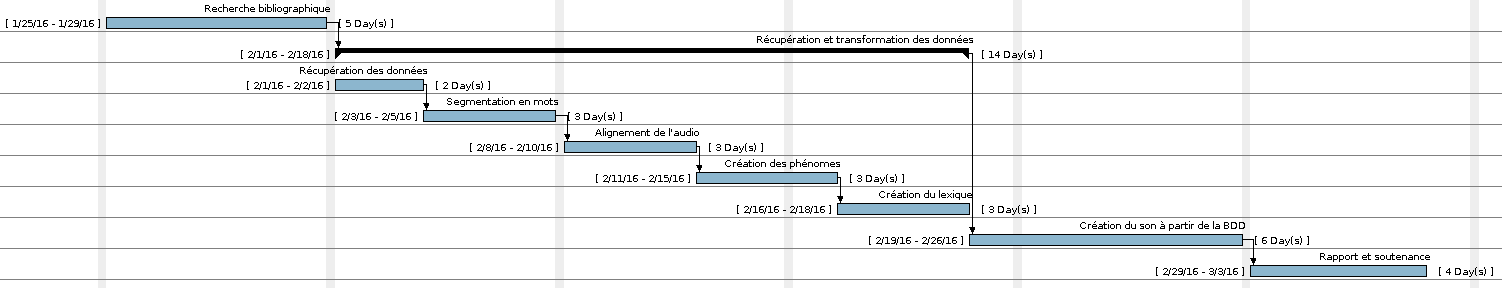
\includegraphics[max size={\textwidth}{\textheight}]{contents/img/gantt.jpg}
		\caption{Diagramme de Gantt}
		\label{Figure:gantt}
	\end{figure}

	\section*{Conclusion}

	Le projet consiste donc dans un premier temps à générer une correspondance mot/son
	à partir d'audio-books. Nous ne pourrons pas traiter tous les audio-books, nous
	ferons nos expérimentations sur un échantillon beaucoup plus réduit.
	
	Plusieurs approches sont envisageables, on retiendra une analyse du signal, un
	apprentissage non supervisé~\cite{ludusan:hal-01026368} et un autre 
	supervisé~\cite{Panayotov2015}.
	
	Puis il s'agit simplement d'utiliser la base de donnée générée pour produire 
	un son.